\section{Performance of Individual Mitigations}
\label{s:evolution-eval}

This section explores in more detail the individual mitigations that contributed
to the previously shown end-to-end overheads.
Our aim is to understand why some mitigation costs have gone down while others have not.

For each mitigation, we attempt to isolate the relevant instruction sequence and examine what the cost is on each of our processors.
To achieve precise timings, we rely on the timestamp counter functionality available on x86 and average over one million runs to eliminate noise.

\subsection{Meltdown}

On LEBench, the Meltdown mitigation accounts for one of the most substantial performance impacts, singlehandedly causing an around 10\% overhead on its own.
On processors vulnerable to Meltdown, production operating systems use page table isolation (PTI) to mitigate it.
This approach adds significant overhead to every user-kernel boundary crossing, because it requires switching the page tables every time via a \texttt{mov} to the \texttt{\%cr3} register.
Among the systems we evaulated, only Broadwell and Skylake are vulnerable to Meltdown.

As seen in Table~\ref{table:meltdown}, on processors vulnerable to Meltdown the cycles required to swap page tables when entering and again on leaving the kernel far exceeds the time for the actual \texttt{syscall} or \texttt{sysret} instruction that triggers the entry/exit.
For syscalls, the Ice Lake Client CPU takes fewer cycles (which will prove a pattern---likely due to its lower base clock speed) and the Cascade Lake model stands out by taking longer than both earlier and later Intel models.

\begin{table}[h]
  \begin{center}
  \begin{tabular}{clccc} 
    \textbf{Vendor} & \textbf{CPU} & \textbf{\texttt{syscall}} & \textbf{\texttt{sysret}}  & \textbf{swap \texttt{cr3}} \\ \hline 
    \multirow{5}{*}{Intel} & Broadwell             & 49 & 40 & 206 \\
                           & Skylake Client        & 42 & 42 & 191 \\
                           & Cascade Lake          & 70 & 43 & 0 \\
                           & Ice Lake Client       & 21 & 29 & 0 \\
                           & Ice Lake Server       & 45 & 32 & 0 \\ \hline
      \multirow{3}{*}{AMD} & Zen                   & 63 & 53 & 0 \\
                           & Zen 2                 & 53 & 46 & 0 \\
                           & Zen 3                 & 83 & 55 & 0 \\ \hline
  \end{tabular}
  \end{center}
  \caption{Average cycles to execute a \texttt{syscall} or \texttt{sysret} instruction, and for vulnerable processors, to swap page tables. }
  \label{table:meltdown}
\end{table}

One other impact of page table isolation is that on old processors it can cause increased TLB pressure due to much more frequent TLB flushes.
Both Broadwell and Skylake Client, however, support PCIDs which tag page table entries with a process identifier.
This means that on those processors the TLB has to be flushed much less often, and makes TLB impacts marginal compared to the direct cost switching the root page table pointer.

\subsection{Microarchitectural Data Sampling}

The other substantial mitigation on LEBench is clearing CPU buffers, which is required to mitigate Microarchitectural Data Sampling (MDS).
On processors that are vulnerable to MDS, a microcode patch extends the \texttt{verw} instruction to also implement this clearing functionality.
Without the patch the \texttt{verw} only has its old behavior related to segmentation.

Table~\ref{table:verw} shows that the cost of performing this flush is approximately 500 cycles.
This cost is substantial because microarchitectural buffers must be flushed not
just on context switches between processes but also on every kernel-to-user privilege transition.
Recent Intel processors and all processors from AMD are not vulnerable to MDS.
On these processors the \texttt{verw} has only its legacy segmentation-related behavior and takes only tens of cycles.

\begin{table}[h]
  \begin{center}
  \begin{tabular}{clc}
      \textbf{Vendor} & \textbf{CPU} & \textbf{Clear Cycles} \\ \hline 
      \multirow{5}{*}{Intel} & Broadwell             & 610 \\
                             & Skylake Client        & 518 \\
                             & Cascade Lake          & 458 \\
                             & Ice Lake Client       & 0 \\
                             & Ice Lake Server       & 0 \\ \hline
      \multirow{3}{*}{AMD}   & Zen                   & 0 \\
                             & Zen 2                 & 0 \\
                             & Zen 3                 & 0 \\ \hline
  \end{tabular}
  \end{center}
  \caption{Cycles required to clear microarchitectural buffers using the
    \texttt{verw} instruction. Processors not vulnerable to MDS are listed as
    zero cycles because they do not require any microarchitectural buffers to be cleared before returning to user space. }
  \label{table:verw}
\end{table}

\subsection{Spectre V2}

Spectre V2 involves poisoning the branch target buffer so that an indirect branch in victim code jumps to a Spectre gadget.
As we saw, mitigating Spectre V2 is a small but largely consistent drag on LEBench performance across all the processors.

\paragraph{Indirect Branch Restricted Speculation}

Indirect Branch Restricted Speculation (IBRS) was the first mitigated proposed for Spectre V2 and is enabled by setting a MSR bit which must be repeated on every entry into the kernel.
Newer Intel processors---Cascade Lake and onward---support extended IBRS (eIBRS), which allows the operating system to enable IBRS once at boot time, and have it remain in effect without additional system register writes.

The cycle cost of doing this MSR write on every system call was viewed as unacceptably high, so production operating systems investigated alternative approaches, ultimately settling on retpolines for any processor not supporting eIBRS.

\paragraph{Retpoline}

Retpolines are the primary software mitigation for Spectre V2 today.
They involve replacing every indirect branch in the kernel with an alternate instruction sequence.
A retpoline sequence has identical behavior to an indirect branch instruction, except that the branch destination (and more importantly any Spectre gadgets) are never jumped to speculatively.

There are a couple variations of retpolines, with slightly different characteristics.
So called ``generic retpolines'' use a code sequence involving a \texttt{call} instruction, a write instruction to replace the saved return address with the jump target, and a \texttt{ret} instruction to cause the processor to speculatively jump back to the call site (due to the return value stack) before correcting to the intended branch target.
This version works on both Intel and AMD processors.

An alternative version ``AMD retpoline'', involves simply doing an \texttt{lfence} followed by a normal indirect branch.
As might be inferred from the name, this variant does not work on Intel: code using it would still be vulnerable to Spectre V2.

\begin{figure}[h]
  \begin{lstlisting}[language={[x86masm]Assembler}]
generic_retpoline:
    call 2f
1:  pause
    lfence
    jmp 1b
2:  mov %r11, (%rsp)
    ret

amd_retpoline:
    lfence
    call *%r11\end{lstlisting}
  \caption{Assembly sequences for the two kinds of retpolines}
  \label{fig:retpoline-samples}
  \end{figure}

Table~\ref{table:retpoline} shows extra cycles of each of these variations across our machines, relative to a baseline of doing an unsafe indirect branch.
One noticeable takeaway is that IBRS adds tens of cycles of overhead to indirect branches except on processors with eIBRS support (Cascade Lake and the two Ice Lake CPUs) where it is inexpensive.
Retpolines however can be as or even more costly.

The AMD processors have different performance executing AMD
retpolines: on the Zen 2 model we measure no overhead compared to a
normal indirect branch, while the other AMD processors they are even
slower than a generic retpoline.

%The main takeaway is consistent with the LEBench results: mitigation costs have remained small but non-trivial across processor generations.




\begin{table}[h]
\begin{center}
\begin{tabular}{ clcccc }
  \textbf{Vendor} & \textbf{CPU} & \textbf{Baseline} & \textbf{IBRS} & \textbf{Generic} & \textbf{AMD} \\ \hline
  \multirow{5}{*}{Intel} & Broadwell           & 16 & +32 & +28 & \tiny{N/A} \\
                         & Skylake Client      & 11 & +15 & +19 & \tiny{N/A} \\
                         & Cascade Lake        & 3 & +0 & +49 & \tiny{N/A} \\
                         & Ice Lake Client     & 5 & +0 & +21 & \tiny{N/A} \\
                         & Ice Lake Server     & 1 & +1 & +50 & \tiny{N/A} \\ \hline
  \multirow{3}{*}{AMD}   & Zen                 & 30 & \tiny{N/A} & +25 & +28 \\
                         & Zen 2               & 3 & +13 & +14 & +0 \\
                         & Zen 3               & 23 & +19 & +13 & +18 \\ \hline
\end{tabular}
\end{center}
\caption{Baseline cycles to perform an indirect branch, and the added cost of doing indirect branches with IBRS enabled, the added cost of an indirect branch via a generic repoline, and via an AMD retpoline.}
\label{table:retpoline}
\end{table}

\paragraph{Indirect Branch Prediction Barrier (IBPB)}

In addition to preventing indirect branches in the kernel from being
hijacked, it is also important that one user process cannot launch a Spectre V2 attack against another process.
To prevent this attack, on every context switch between processes the operating system runs an Indirect Branch Prediction Barrier to clear the branch target buffer.

We verified across all our processors that executing an IBPB between poisoning the branch target buffer and performing an indirect branch prevents execution from being routed to the attacker-controlled target.
Oddly, however, we noticed that the performance counters report that indirect branches executed after an IBPB result in mispredictions.
We speculate that this behavior is caused by the IBPB setting all entries in the BTB to point to a specific harmless gadget rather than simply clearing them.

Table~\ref{table:ibpb} shows that the cost of an IBPB has generally
declined over time from many thousands of cycles on the Broadwell
server to hundreds of cycles on Cascade Lake and Ice Lake Server.
This improvement is likely related to the fact that older processors implemented IBPB via a microcode patch, whereas newer ones may have some amount of support in hardware.
The Ice Lake Client processor somewhat bucks the trend of improving performance when compared to the earlier Cascade Lake, but still requires many fewer cycles than Broadwell or Skylake.
AMD processors we tested show a similar improvement across generations.

\begin{table}[h]
    \begin{center}
    \begin{tabular}{ clc }
      \textbf{Vendor} & \textbf{CPU} & \textbf{IBPB cycles} \\ \hline

      \multirow{5}{*}{Intel} & Broadwell         & 5573 \\
                             & Skylake Client    & 4537 \\
                             & Cascade Lake      & 340 \\
                             & Ice Lake Client   & 2455 \\
                             & Ice Lake Server   & 836 \\ \hline
      \multirow{3}{*}{AMD}   & Zen               & 7370 \\
                             & Zen 2             & 1088 \\
                             & Zen 3             & 808 \\ \hline
    \end{tabular}
    \end{center}
    \caption{Cycles to execute an indirect branch speculation barrier. }
    \label{table:ibpb}
\end{table}

\paragraph{Return Stack Buffer Filling}

When a user process employs generic retpolines to protect itself from Spectre V2, it is counting on the return stack buffer not being tampered with during the code sequence.
Unfortunately, if the operating system triggers a context switch at an inopportune time then this condition might be violated.
Linux uses two approaches to guarantee that user-level retpolines still work despite interrupts potentially happening at any time during execution.

The first is a static analysis pass over the Linux kernel at build time to ensure that the operating system itself doesn't have  unbalanced \texttt{call} and \texttt{ret} pairs anywhere, which incurs no runtime cost at all.
Since any code compiled with the regular toolchains will already have this property, this check is not expected ever to fail.

Secondly, when context switching between different user threads Linux will fill the the return stack buffer with harmless entries.
This is required so that any interrupted retpoline sequence will avoid jumping to any Spectre gadgets---meaning that despite not causing a speculative jump to the intended retpoline landing point, it will still produce safe results.

Table~\ref{table:rsb-fill} shows the cycles required to fill the return stack buffer on each processor.
There is improvement across generations of Intel processors but less of a clear trend across the AMD CPUs.
These changes are likely realized more by improving performance overall
than trying to optimize for return stack buffer filling specifically, but regardless, the cost of these mitigations is relatively minor compared to the total overhead of doing a context switch between processes (which takes at least several thousand cycles)

\begin{table}[h]
  \begin{center}
  \begin{tabular}{clc}
      \textbf{Vendor} & \textbf{CPU} & \textbf{RSB Fill Cycles} \\ \hline
      \multirow{5}{*}{Intel} & Broadwell       & 130 \\
                             & Skylake Client  & 130 \\
                             & Cascade Lake    & 120 \\
                             & Ice Lake Client & 40 \\
                             & Ice Lake Server & 69 \\ \hline
      \multirow{3}{*}{AMD}   & Zen             & 114 \\
                             & Zen 2           & 68 \\
                             & Zen 3           & 94 \\ \hline
  \end{tabular}
  \end{center}
  \caption{Cycles to stuff the RSB. }
  \label{table:rsb-fill}
\end{table}

Return stack buffer filling also provides protection against variations of
SpectreRSB~\cite{koruyeh:spectrersb}, which exploits the return stack buffer itself.
Thus while the overall toggle to enable the functionality is controlled by Linux's \texttt{nospectre\_v2} option, some amount of the overhead attributed to Spectre V2 should probably be accounted to mitigating SpectreRSB instead.

\subsection{Spectre V1}

On the Octane 2 benchmarks, the various Spectre V1 mitigations collectively accounted for a large fraction of the total overhead.
We discuss each of them in more detail.

\paragraph{lfence}

One mitigation for Spectre V1 is to execute an \texttt{lfence} instruction immediately following each bounds check and \texttt{swapgs} instruction.
This instruction waits until all prior loads have resolved, thereby preventing any subsequent Spectre gadget from executing.
The cost of an \texttt{lfence} varies significantly based on operations in flight.
Table~\ref{table:lfence} shows the results of a simple microbenchmark of running an \texttt{lfence} instruction in a loop.
An important caveat is that the performance will depend a lot on what other instructions have been executed prior so this is not a fully representative experiment.

We see that all times are roughly of the same scale, with newer processors showing better performance.
The \texttt{lfence} does more work on AMD than on Intel (as evidenced by the AMD retpoline sequence described earlier) so the numbers are not directly comparable across vendors.

\begin{table}[h]
  \begin{center}
  \begin{tabular}{ clc }
    \textbf{Vendor} & \textbf{CPU} & \textbf{lfence cycles} \\ \hline
    \multirow{5}{*}{Intel} & Broadwell        & 28 \\
                           & Skylake Client   & 20 \\
                           & Cascade Lake     & 15 \\
                           & Ice Lake Client  & 8 \\
                           & Ice Lake Server  & 13  \\ \hline
    \multirow{3}{*}{AMD}   & Zen              & 48 \\
                           & Zen 2            & 4 \\
                           & Zen 3            & 30 \\ \hline
  \end{tabular}
  \end{center}
  \caption{Cycles to execute a single lfence instruction on each machine.
    In real applications, the cost will heavily depend on the other loads in flight. }
  \label{table:lfence}
\end{table}

\paragraph{Index Masking}

Instead of preventing speculation past bounds checks, an alternative mitigation is to force the array index to zero for any out of bounds access.
SpiderMonkey (the JavaScript engine used by Firefox) uses this
strategy: before every array indexing operation it inserts a
\texttt{cmov} instruction that overwrites the array index with zero if it would be past the end of the array.
Unlike in many compiled languages, JavaScript always knows the lengths of arrays so this mitigation can be applied automatically to the generated assembly.
On the committed execution path the conditional move will always be a no-op (because as a safe language JavaScript always does bounds checks), but in the speculative case it blocks execution until the array length has resolved.
Our measurements of the Octane 2 benchmark suite indicate this approach incurs an approximately 4\% performance overhead.

\paragraph{Object Mitigations}

Since JavaScript is dynamically typed, the compiler must insert many runtime checks on the types of variables.
This presents another possible avenue for Spectre V1 attacks, because mis-speculating an object's type can cause its fields to be misinterpreted, potentially resulting in out of bounds memory reads.
The mitigation is similar to index masking: object guards insert a conditional move that zeros out the object pointer if the check check fails.
This mitigation incurs an overhead on Octane 2 on the order of 6\%.

\subsection{Speculative Store Bypass}
\label{sec:ssb}

\begin{figure}[h]
  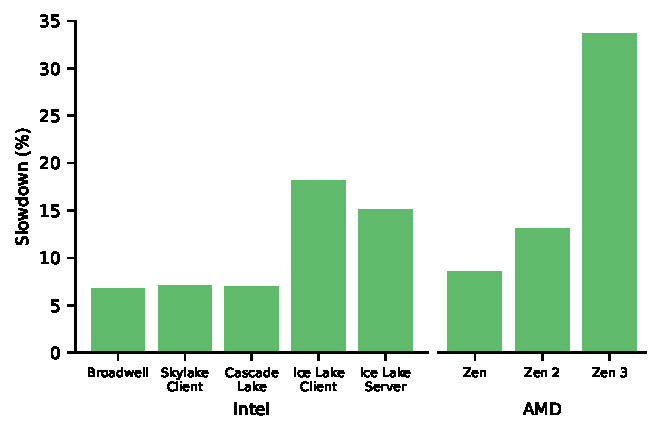
\includegraphics[width=\columnwidth]{plots/ssbd.pdf}
  \caption{The slowdown caused by Speculative Store Bypass Disable on three benchmarks from the PARSEC suite.}
  \label{fig:ssbd}
\end{figure}

Speculative Store Bypass, originally called Spectre V4, exploits the processor's store-to-load forwarding to enable an attacker to learn the contents of recently written memory locations.
The only available defense against the attack is to enable a processor mode called Speculative Store Bypass Disable (SSBD) that blocks this forwarding.
A downside is that this can come at substantial cost, even when normal non-malicious code is being run.

The compromise reached by the Linux developers was to enable SSBD only for processes which opted into it via its \texttt{prctl} or \texttt{seccomp} interfaces.
To see the full impact of this mitigation if enabled all the time, we measured the slowdown it causes to the swaptions benchmark from PARSEC.
Figure~\ref{fig:ssbd} shows that the slowdown can be as much as 34\%,
and is trending worse over time.
It isn't entirely clear why this would be the case, but it may be related to newer processors have a more complete SSBD implementation compared to what was possible via microcode patches.
These overheads are especially considerable given that the combined
impact of all default mitigations for this benchmarks is well under one percent (\S\ref{sec:benchmarks:parsec}).

\subsection{L1 Terminal Fault}
One other attack worth mentioning is L1 Terminal Fault, which can leak the entire contents of the L1 cache when page tables contain PTEs with certain bit patterns.
Linux avoids ever creating such PTEs, which can be done with essentially no overhead.
This is consistent with it not showing up in our end-to-end performance study earlier.

However, the problem is more severe when virtual machines are involved because an untrusted guest operating system could insert such specially crafted PTEs into its own page table.
Doing so would enable it to learn L1 cache contents lingering from memory accesses done by the host, and so the necessary mitigation on vulnerable processors is for the host to flush the L1 cache prior to entering a guest virtual machine.

Our benchmarking of virtual machine workloads did not show any measurable impact from enabling this mitigation and it has also been patched on newer processors, so the relevance should be minimal going forward.

\subsection{Other attacks}

The attacks discussed so far are hardly the only transient execution attacks discovered.
Many others like FPU Register Bypass, System Register Read, and so forth have commanded significant time and attention for computer architects, operating system developers, and security researchers.
However, the cost they incur on workloads today seems to be minimal, so we skip evaluating them individually.
